\begin{tikzpicture}[remember picture, scale=\modDGHyperScale]
% dummy
\coordinate[overlay] (v-coord-0-0) at (0.97227, 0.30073) {};
\coordinate[overlay] (v-coord-1-0) at (2.9828, 0.3) {};

% id = 0, graphName = glycolaldehyde
\node[modStyleDGHyperVertex, at=(v-coord-0-0)] (v-0-0) {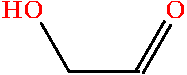
\includegraphics[scale=\modDGHyperImageScale] {\modInputPrefix/out/008_g_0_11311100.pdf}\\{$\mathrm{glycolaldehyde}$}};
% id = 1, graphName = p_{0,0}
\node[modStyleDGHyperVertex, at=(v-coord-1-0)] (v-1-0) {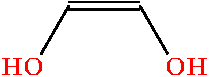
\includegraphics[scale=\modDGHyperImageScale] {\modInputPrefix/out/010_g_1_11311100.pdf}\\{$\mathrm{p_{0,0}}$}};
% id = 2{ 'glycolaldehyde' }, 'Keto-enol', { 'p_{0,0}' }
\path[modStyleDGHyperConnector] (v-0-0) to[modStyleDGHyperHasReverseShortcut] node[auto, swap] {$\mathrm{r_{0}}$} (v-1-0);
% id = 3{ 'p_{0,0}' }, 'Keto-enol, inverse', { 'glycolaldehyde' }
\path[modStyleDGHyperConnector] (v-1-0) to[modStyleDGHyperHasReverseShortcut] node[auto, swap] {$\mathrm{r_{1}}$} (v-0-0);
\end{tikzpicture}%
